\documentclass[11pt]{article}  % min is 11pt
\title{Enhancement and Maintenance of the scikit-learn project\vspace{-3ex}}
\date{\vspace{-5ex}}

\usepackage[margin=1in]{geometry}  % min is .5 in
\usepackage[shortlabels]{enumitem}
\usepackage{graphicx}
\usepackage[hidelinks]{hyperref}
\usepackage{caption}

\begin{document}

\maketitle
\section{Goals}

% 30+ citations but mostly neuro science:
% Large-scale automated identification of mouse brain cells in confocal
% light sheet microscopy images.


The goal of this proposal is to add key features to the open-source machine learning library scikit-learn and aid in maintaining the project.

Scikit-learn powers many applications of machine learning and data science,
and it is used in many bio-medical
applications~\cite{roles_of_ml_in_biomed_science} including neuroscience~\cite{zandifar2017comparison, valera2016stereotyped, spike_sorting}, pharmaceutics~\cite{lindh2017predicting, lorberbaum2015systems, segler2017generating}, psychiatry~\cite{schmidt2015approaching, 10.1001/2013.jamapsychiatry.5, patel2015machine}, cancer research~\cite{bakas2017advancing, TAYLOR2018676, chaudhary2018deep}, epigenetics~\cite{wang2017epigenetic, kakaradov2017early, dogan2018integrated}, radiology~\cite{masino2016temporal,wang2015evaluation} and genetics~\cite{LAMANNO2016566, horlbeck2016compact, brannan2016sonar}. Thanks to its ease of use, scikit-learn enables domain scientists without extensive machine learning knowledge to efficiently apply machine learning techniques to their core
discipline; as a result, the original scikit-learn paper~\cite{scikit-learn} has more
than 18,000 citations, and the GitHub repository\footnote{\href{https://github.com/scikit-learn/scikit-learn}{https://github.com/scikit-learn/scikit-learn}} is used by more than 62,000 repositories. It is also a core upstream dependency of more
specialized packages like Starfish\footnote{\href{https://github.com/spacetx/starfish}{https://github.com/spacetx/starfish}} for transcriptomics, Scanpy~\cite{scanpy} for single-cell analysis, or CellProfiler~\cite{cellprofiler} for biological image analysis which are directly built or funded by CZI. Other downstream packages include
QIIME~\cite{QIIME2, QIIME2_feature_classifier,
QIIME2_sample_classifier}, Nilearn~\cite{Neuro_imaging_sklearn}, MNE~\cite{MNE},
Scikit-allel\footnote{\href{https://github.com/cggh/scikit-allel}{https://github.com/cggh/scikit-allel}},
MSMBuilder~\cite{MSMBuilder}, or MOABB~\cite{MOABB}.

This proposal aims to fund the work of Andreas M\"uller (PI) for 4.5 months,
and that of Nicolas Hug (co-PI) for 12 months. M\"uller and Hug are both
associate research scientists at Columbia University. M\"uller has been a
core-developer of scikit-learn for over 7 years, and Hug has been a core
developer for about six months. We plan to address the following tasks,
detailed in the next subsections:
\begin{itemize}
\item Maintenance of the library and removal of technological debt
\item Improvements to the new fast gradient boosting models
\item Faster parameter searches, avoiding redundant computations
\end{itemize}

\subsection{Maintenance of the library}

As one of the most widely used machine learning libraries, scikit-learn has
a tremendously large code-base, of which some parts are many years old. New contributions are submitted each day, along with many bug reports or
feature requests. We propose to fund both M\"uller and Hug to ensure the
continued improvement of the library, and to ensure the project evolves to
meet the growing needs of the scientific community. Maintaining scikit-learn consists of:

\begin{enumerate}[a)]
\item Addressing bug reports, prioritizing bug fixes, and ensuring important bugs are fixed in a timely manner.
\item Reviewing new feature contributions and making sure they meet the high
quality criteria of the project, in particular regarding code
maintainability and user documentation.
\item Supporting and connecting with the community: this includes
maintaining a high-quality documentation, reaching out to users to advertise
new useful features, and decide what directions to take according to community
needs. It also involves organizing sprints to engage the community and
increase diversity among the contributors.
\item Making sure backward compatibility is preserved between versions, and
that new features are consistent with the needs of the library. This is
important for the health of the project and for the numerous downstream
projects that rely on scikit-learn.
\item Reducing the current backlog. There are many issues and pull-requests that get stalled for various reasons. Reviewing these pull requests and closing irrelevant ones helps contributors and developers to focus on important matters.
\end{enumerate}

These tasks require experience and a consistent involvement in the project
to be carried out efficiently, making the team of M\"uller and Hug
particularly well suited for this task.

\subsection{Improvements to Gradient Boosting}

Gradient Boosting Decision Trees (GBDTs) are a family of machine learning
models used for classification and regression tasks. GBDTs are extremely
efficient and often out-perform other models. They are used pervasively in
machine learning, including biomedical applications~\cite{chen2019hiv, shah2019development}.

Recent implementations like LightGBM~\cite{LightGBM} and XGBoost~\cite{XGB}
offer state-of-the-art results, both in terms of prediction accuracy and
computation time. However, directly including an implementation in scikit-learn ensures compatibility with the core package, and prevents inconsistencies in the API. Moreover, due to scikit-learn's popularity, distributing an implementation with scikit-learn will increase the visibility and adoption of these highly effective algorithms by non specialists.

A new implementation of GBDTs (by co-PI Hug) was recently
released in scikit-learn version 0.21. This new implementation
outperforms XGBoost in terms of speed (while matching it's accuracy), and its results (in terms of speed and accuracy)
are on a par with LightGBM. While the current implementation is operational,
several important features are not implemented yet. Therefore we propose the following enhancements to this new GBDT implementation:
\begin{enumerate}[a)]
\item Implement native support for missing values. In real-world datasets, feature values might be missing due to measurement errors or incomplete measurements. In these cases, practitioners need to resort to
imputation, which is often sub-optimal and not theoretically grounded~\cite{missing_values_consistency}.
Unlike most machine learning models, GBDTs are able to natively support
missing data, without resorting to imputation of missing values. This makes
them extremely handy to use, in particular for non-specialists. Both
LightGBM and XGBoost natively support missing values.
\item Implement native support for categorical features. Categorical
features are pervasive in bio-medical science. For example sex, age, race,
or geographic location are potentially relevant
for predicting the cancer risk of a patient \cite{RICHTER201929}, and could be encoded as categorical variables. The current
implementation of GBDTs only supports continuous features, but GBDTs are
also able to handle categorical data. For now, users are required to
preprocess categorical features using techniques like one-hot-encoding, which
is often tedious and can lead to worse results. GBDTs have a native, more efficient way of dealing with categorical variables. 
Implementing this would free practitioners from having to worry about encoding categorical variables.
This feature is implemented in LightGBM, but not in XGBoost.
\item Implement support for sample weights and class weights, which allow the user to specify the confidence they have in their measurements and deal with imbalanced datasets.
\item Document and explain the usage of the new implementation, with an emphasis on missing value support and support for categorical variables. Create detailed examples of typical use-cases.
\item Maintain the code, and fix the potential bugs. The current
implementation already has about 5000 lines of Python (and Cython) code.
Despite great efforts to provide a thorough test suite, some bugs or
numerical instability issues may still be present, which is expected for a
code base of that size and complexity.

\item Improved scalability on multiple cores. The new GBDT implementation is our first use of low-level
parallelism (using OpenMP). This enables us to build extremely
efficient estimators, but requires careful engineering and benchmarking to take full advantage of modern multi-core systems.
\end{enumerate}

Please also note that achieving a) and b) would make these models the
first ones in scikit-learn to natively support missing data and
categorical data. This will demand some careful design steps, and will increase the number of potential bugs and pitfalls.


\subsection{Faster parameter searches avoiding redundant computations}

Supervised machine learning workflows typically consist of one or multiple
preprocessing steps, and a final supervised model. The preprocessing steps, as well as the final model, commonly have hyper-parameters that need to be tuned
for the overall procedure to perform well on a specific task: this is called a
hyper-parameter tuning. Scikit-learn provides tools for hyper-parameter tuning: namely grid search (exhaustively try parameter combinations along a grid) and
random search (parameter combinations are sampled at random).

Performing parameter searches in machine learning workflows often involves
redundant computation, and previously computed results can potentially be
re-used. As illustrated on Figure \ref{fig:fast_grid_search}, when parameters of
the final model change, it is unnecessary to recompute the previous
(preprocessing) steps.

Currently scikit-learn unnecessarily performs redundant computations, wasting
computation time.

Leveraging dask features, in particular dask’s graph execution engine, the
dask-ml package now provides equivalent implementations of
parameter search logic that are able to re-use previously computed steps.
This implementation can be much faster than the implementation available in
scikit-learn. However, this package is not as popular as the scikit-learn
library, and as a result it is much less likely to be widely used, despite
its usefulness. It also relies on dask, adding a dependency and increasing
maintenance burden. Having such a utility in scikit-learn would allow
non-specialists to train complex pipelines much more efficiently.

We propose to implement parameter search utilities without re-computation
within scikit-learn, taking advantage of experience from the dask-ml
implementation. This is a complex task that may require intrusive changes to
scikit-learn core utilities.

\subsection{Expected outcomes, success evaluation and metrics}
For open source projects, measuring impact is notoriously hard, as library authors don't have access to telemetry. Download counts are often spread over several distribution channels and highly skewed by automated downloads. The impact of specific additions to open source projects is even harder to measure, in particular since adoption of new features can only be measured with significant delay. Acknowledging this, we are suggesting proxy metrics that allow at least some quantitative evaluation of the work in the Milestones and Deliverables document.

\subsubsection{New features for GBDT models}

For the GBDT models, our primary goal is merging the proposed
features (in particular support for missing values and categorical data) into scikit-learn, and inclusion into a release of the package. We also expect our additions to increase usage of the HistGradientBoosting models, as can be measured by code search on Github. Currently a search for Jupyter Notebook returns about 50 hits, we expect this to rise to over 200.

\subsubsection{Faster parameter searches}

Given the complexity of the
task, such an implementation would require some careful design steps. There
are indeed many different approaches to solving this problem, each of which
has its own technical constraints. As a result, clearly defining and
assessing the pros and cons of each approach would already be an
accomplishment and would serve as groundwork for future directions.

Our goal would be successfully met here if we can reach a consensus on implementation path. A release of the implementation would be a stretch goal.

\section{Work plan}


The funds would be used to:
\begin{itemize}
\item Fund Andreas M\"uller's position for 4.5 months. His long-term experience with the project is essential for evaluating changes in API design and dependencies that are necessary for the planned work.
\item Fund Nicolas Hug's position for 12 months. Hug has been involved in
maintaining scikit-learn for over a year, and has been a core developer for 6 months. He has contributed key features
to the package, in particular the new GBDT implementation mentioned above.
\item Fund participations in some key Python and scientific conferences,
such as the SciPy conference
\footnote{\href{https://conference.scipy.org/}{https://conference.scipy.org}}.
\item Fund participation and organization of sprints, in particular the WiMLDS sprints\footnote{\href{http://wimlds.org/opensourcesprints-2/}{http://wimlds.org/opensourcesprints-2/}}. See our \textit{Diversity and Inclusion Statement} for details on these events.
\end{itemize}

We believe that mentoring other contributors is very important for the
health of the project: the more contributors are familiar with the code
base, the healthier the project. Therefore, a significant part of the effort in
implementing the proposed features will go towards reviewing and
mentoring other contributors, instead of implementing all of the features
ourselves.

All of the proposed features in this proposal are part of the current
project
roadmap\footnote{\href{https://scikit-learn.org/stable/roadmap.html}{https://scikit-learn.org/stable/roadmap.html}}.


\section{Existing support}

 Andreas M\"uller is a PI on the following grants related to scikit-learn:

\begin{itemize}
    \item \textit{Building blocks and Search Improvements for Automated Machine Learning Model Selection}. DARPA. \$351k.  2018.
    \item SI2-SSE: \textit{Improving Scikit-learn usability and automation}. NSF. \$400k.  2017-2020.
    \item \textit{Extension and Maintenance of Scikit-learn}. Alfred P. Sloan Foundation. \$313k.  2017-2019.
\end{itemize}


The scikit-learn foundation at INRIA Paris
\footnote{\href{https://scikit-learn.fondation-inria.fr/}{https://scikit-learn.fondation-inria.fr/}}
currently funds four full time employees working on scikit-learn and related
projects:
\begin{itemize}
\item Olivier Grisel, technical lead.
\item J\'er\'emie du Boisberranger, research engineer.
\item Guillaume Lema\^itre, research engineer.
\item Chiara Marmo, community and operation manager (starting September 2019).
\end{itemize}

The University of Sydney funds Joel Nothman to work part-time on
scikit-learn.
Anaconda\footnote{\href{https://www.anaconda.com/}{https://www.anaconda.com/}}
funds Adrin Jalali as a full time employee to work on scikit-learn and
related projects.

\clearpage
\section*{Figures}

\begin{figure}[h!]
  \centering
    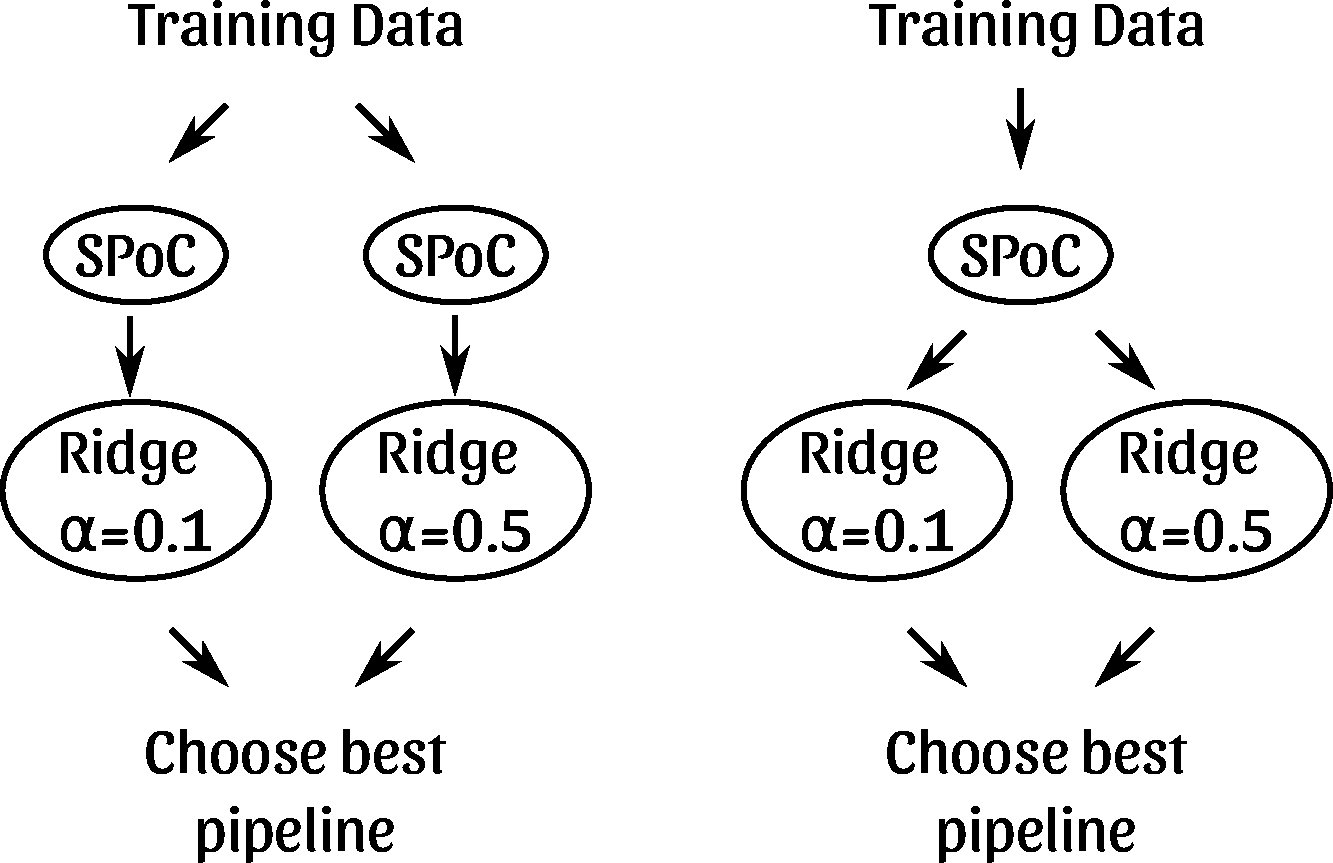
\includegraphics[width=0.5\textwidth]{drawing}
  \caption{
      Parameter search for a model predicting electromyography signal
      from magnetoencephalography activity. Inspired by the MNE
      package\cite{MNE}.\\
      \textbf{Left}: Current parameter search in
      scikit-learn. The pre-processing SPoC step is repeated for each of the
      two pipelines, even though it never changes.\\
      \textbf{Right}: Proposed implementation. The SPoC step is only
      computed once.
      }
      \label{fig:fast_grid_search}
\end{figure}

\clearpage
\bibliographystyle{abbrv} % or named ?
\bibliography{biblio}

\end{document}
